\documentclass[12pt]{article}
\usepackage{xcolor}
\usepackage[latin]{babel}
\usepackage[utf8]{inputenc}
\usepackage[T1]{fontenc}
\usepackage{amsmath}
\usepackage{amsfonts}
\usepackage{amssymb}
\usepackage[version=4]{mhchem}
\usepackage{stmaryrd}
\linespread{1.5}
\setlength{\parindent}{0pt}
\usepackage{listings}
\usepackage{xcolor}
\usepackage{algorithm}
\usepackage{algpseudocode}
\usepackage{tikz}
\usepackage{pifont}
\begin{document}
$\text{A}_{1}$

$\text{Q}_{1}$

1. True

PF: WTS: $\exists c_{1}, c_{2} \in R^{+}, \exists n_{0} \in N, \forall n \in N\left[n \geq n_{0} \Rightarrow c_{1} \cdot n^{2} \leq 9 n^{2}+5 n-17 \leq c_{2} n^{2}\right]$


Choose $c_{1}=8, c_{2}=14, n_{0}=4$

Consider $n$ be an arbitrary number of $N$

Suppose $n \geq 4$, we have,

$
\begin{array}{rlrl}
9 n^{2}+5 n-17 & >8 n^{2}+5 n-17 & & \left(9 n^{2}>8 n^{2} \text { if } n \geq 4\right) \\
&>8 n^{2} & & (5 n-17 \geq 0 \text { if } n \geq 4) \\
9 n^{2}+5 n-17 & <9 n^{2}+5 n & & (-17<0) \\
& <9 n^{2}+5 n^{2} & & \left(5 n^{2}>5 n \text { if } n \geq 4\right) \\
& =14 n^{2} & & \\
\Rightarrow 8 n^{2} \leq 9 n^{2}+5 n-17 \leq 14 n^{2} & &
\end{array}
$

As $n$ is an arbitrary number,
\begin{equation*}
9 n^{2}+5 n-17 \in \theta\left(n^{2}\right)
\end{equation*}

QED

2. True

PF: WTS: $\exists c_1 \in R^{+}, \exists n_{0}\in N, \forall n \in N\left[n \geq n_{0} \Rightarrow n \log (n) \leq c_1 n^{2}\right]$

Choose $c_{1}=1, n_{0}=10$

Consider $n$ be an arbitrary number of $N$

Suppose $n \geq 10$

We have $n \log (n)<n\cdot n=n^2 \quad(n>\log (n)>0$ if $n \geq 10)$ 

$\Rightarrow n \log (n) \leq n^{2}$

As $n$ is an arbitrary number of $R$,

$n(\log n) \in O{\left(n^{2}\right)}$

QED.

3. False

PF: WTS: $\forall c_1 \in R^{+}, \forall n_{0} \in N, \exists n \in N\left[n \geq n_{0} \wedge n^{2}>c_1 n\log (n)]\right.$

Consider $c_{1}, n_{0}$ be arbitrary number from $R^{+}$and $N$.

Choose $n$ to be $\max \left(n_{0}, 10^{\left\lceil c_1\right\rceil+5}\right) \in N$

Then we have $n \geq n_{0}>0  \wedge n \geq 10^{\left\lceil c_1\right\rceil+5}$

Consider $h(n)=\frac{n}{\log (n)} \quad(n \geq 5)$

$
\begin{aligned}
h(n)^{\prime} & =\left(\log (n)-n \cdot \frac{1}{n \ln {(10)}}\right) / \log ^{2}(n) \\
& =\left(\log (n)-\frac{1}{\ln {(10)}}\right) / \log ^{2}(n)\\
&>0 \quad \text{if}~n \geq 5
\end{aligned}
$

As $10^{\left\lceil c_1\right\rceil+5}>10^{5}>5 \wedge n \geq 10^{\left\lceil c_1\right\rceil+5}>5$ 

$
\begin{aligned}
h(n) & = \frac{n}{\log n} \\
& \geq \frac{10^{\left\lceil c_1\right\rceil+5}}{\left\lceil c_1\right\rceil+5} \\
& > \frac{(\left\lceil c_1\right\rceil+5)^2}{\left\lceil c_1\right\rceil+5} & & (\forall  n \in R^+, 10^n > n^2)\\
& = \left\lceil c_1\right\rceil+5 \\
&> c_1\\
\end{aligned}
$

$ \Rightarrow \frac{n}{\log (n)}>c_{1}$ 


As $n>5, \quad \log (n)>0$

$
\begin{aligned}
& \Rightarrow n>c_{1} \log (n) \\
& \Rightarrow n^{2}>c_{1} n \log (n) \\
& \therefore n \geq n_{0}, n^{2}>c_1 n\log (n), \text { as wanted } \\
& \Rightarrow n^{2} \notin O(n  \log (n)) \\
\end{aligned}
$

QED.

4.True


PF: WTS: $\exists c \in R^{+}, \exists n_{0} \in N, \forall n \in N\left[n \geq n_{0} \Rightarrow \log \left(n^{2025}+n+1 \leq c \log (n)\right]\right.$

Choose $c=2026, n_{0}=2$

Consider $n$  to be an arbitrary number $\in N$

Suppose $n \geq n_{0}=2$

Consider $g({n}) =n^{2026}-n^{2025}-n-1 \quad(n \geq 2)$

$
\begin{aligned}
& g^{\prime}(n)=2026 n^{2025}-2025 n^{2024}-1 \\
&=n^{2024}(2026 n-2025)-1 \\
& n^{2024}(2026 n-2005)>n^{2024} \geq 2^{2024}>1 \\
& \therefore g^{\prime}(n)>0 \quad(n \geq 2)
\end{aligned}
$

$
\begin{aligned}
& \therefore g(n)>g(2)=2^{2026}-2^{2025}-2-1>0 \quad(n \geq 2) \\
& \therefore n^{2026}>n^{2025}+n+1>0 \\
& \therefore \log \left(n^{2026}\right)>\log \left(n^{2026}+n+1\right) \\
& \therefore \log \left(n^{2025}+n+1\right)<\log \left(n^{2026}\right)=2026 \log (n) \\
& \therefore \log \left(n^{2025}+n+1\right) \leq 2026 \log (n), \text { as wanted }
\end{aligned}
$

As $n$ is an arbitrary number,
\begin{equation*}
\log \left(n^{2025}+n+1\right) \in O(\log (n))
\end{equation*}

QED.

5.False


PF: WTS: $\forall c \in R^{+}, \forall n_{0} \in N, \exists n \in N\left[n \geq n_{0} \wedge(n+1)!>c \cdot n!\right]$

Consider $c\in {R }^{+}, n_{0} \in N$ to be arbitrary numbers.

Choose $n=\max$ ($n_{0}$, $\left\lceil c\right\rceil$)

$
\begin{aligned}
&\Rightarrow  n \geq n_{0}, n \geq\left\lceil c\right\rceil \\
& (n+1)!=n+1 \cdot n!\geq(\left\lceil \bar c\right\rceil+1)-n!>c\cdot n!\text {, as wanted } \Rightarrow(n+1)! \notin O(n!)
\end{aligned}
$

QED
\newpage
$\text{Q}_{2}$

1. False

PF: WTS: $\exists f, g \in N \rightarrow R^{+}, f(n) \notin O(g(n)) \wedge g(n) \notin O(f(x))$ 

Choose $f(n)=\left\{\begin{array}{ll}n & n \text { is even } \\ 1 & n \text { is odd }\end{array} \quad g(n)= \begin{cases}1 & n \text { is even } \\ n & n \text { is odd }\end{cases}\right.$

WTS: $\forall c \in R^{+}, \forall n_{0} \in N, \exists n_{1}, n_{2} \in N$,

$\left[\left(n_{1} \geq n_{0} \wedge f\left(n_{1}\right)>c g\left(n_{1}\right)\right) \wedge(n_{2} \geq n_{0} \wedge g\left(n_{2}\right)>c f\left(n_{2}\right)\right)]$

Consider $c \in R^{+}, n_{0} \in N$ to be an arbitrary number.

Choose $u_{1}=2\left\lceil c\right\rceil\left(n_{0}+1\right), u_{2}=1+2\left\lceil c\right\rceil\left(n_{0}+1\right)$

$\left(n_{1}=2 \left\lceil c\right\rceil(n+1) \geq 2\left(n_{0}+1\right)>n_{0}, n_{2}>n_{1}>n_{0}\right) \Rightarrow\left(n_{1} \geq n_{0}, n_{2} \geq n_{0}\right)$

$f\left(n_{1}\right)=2\left\lceil c\right\rceil\left(n_{0}+1\right)>\left\lceil c\right\rceil>c \cdot 1=c \cdot g\left(n_{1}\right)$, as wanted

$g\left(n_{2}\right)=1+2\left\lceil c\right\rceil\left(n_{0}+1\right)>\left\lceil c\right\rceil>c \cdot 1=c \cdot f\left(n_{2}\right)$, as wanted

QED

2. True:

PF: Consider $f_{1}, f_{2}, g_{2}, g_{2}$ be arbitrary functions $\in N \rightarrow R^{+}$

Suppose $f_{1} \in O\left(g_{1}\right) \wedge f_{2} \in O\left(g_{2}\right)$

we have
$\exists c_{1} \in R^{+}, \exists n_{0} \in N, \forall n \in N\left[n \geq n_{0} \Rightarrow f_{1}(n) \leq c_{1}g_1(n)\right]$

$
\exists c_{2} \in R^{+}, \exists n_{1} \in N, \forall n \in N \left[n \geq n_{1} \Rightarrow f_{2}(n) \leq c_{2} g_{2}(n)\right]
$

WTS: $\exists c_{3} \in R^{+}, \exists n_{2} \in N, \forall n \in N$

$\left[n \geq n_{2} \Rightarrow f_1(n)+f_2(n) \leq c_{3}\left(g_{2}(n)+g_{2}(n)\right)\right]$

Consider $n$ be an arbitrary number from $N$

$
\Rightarrow \exists c_{1}, c_{2} \in R^{+}, n_{0}, n_{1} \in N,$ 

$\text { s.t.}\left(n \geq n_{0} \Rightarrow f_{1}(n) \leq c_{1} g_{1}(n)\right) \wedge\left(n\geq n_{1} \Rightarrow f_2(n) \leq c_{2} g_{2}(n)\right)
$

Choose $c_{3}=\max \left(c_{1}, c_{2}\right) \quad n_{2}=\max (n_0, n_1)$

Suppose $n \geq n_{2}$

$
\begin{aligned}
\Rightarrow & n \geq n_{2} \geq n_{0},  n \geq n_{2} \geq n_{1},  c_{3} \geq c_{1}, c_{3} \geq c_{2} \\
\Rightarrow & f_{1}(n) \leq c_{1} g_{1}(n) \leq c_{3} g_{1}(n) \quad\left(g_{1}(n)>0 \wedge c_{1}>0\right) \\
& f_{2}(n) \leq c_{2} g_{2}(n) \leq c_{3} g_{2}(n) \quad\left(g_{2}(n)>0 \wedge c_{2}>0\right) \\
\Rightarrow & f_{1}(n)+f_{2}(n) \leq c_{3} g_{1}(n)+c_{3} g_{2}(n)=c_{3}\left(g_{1}(n)+g_{2}(n)\right), \text { as wanted }
\end{aligned}
$

QED.

3. False


PF: WTS: $\exists f, g \in N \rightarrow R^{+}, f \in O (g) \wedge 2^{f} \notin O(g)$

Choose $f(n)=2 n, g(n)=n$

WTS: $\exists c_{1} \in R^{+}, \exists n_{0} \in N, \forall n \in N\left[n \geq n_{0} \Rightarrow 2 n \leq c_1 n\right]$

$\wedge \forall c_{2} \in R^{+}, \forall n_1 \in N, \exists n^{\prime} \in N\left[n^{\prime} \geq n_{1} \wedge 2^{2 n^{\prime}}>c_{2} 2^{n^{\prime}}\right]$

Consider $n$ be an arbitrary number from $N$

Choose $c_1=3, n_{0}=1$

Suppose $n \geq n_{0}=1, 2 n<3 n=c_1 n$, as wanted

Consider $c_{2} \in R^{+}, n_1 \in N$ be arbitrary numbers.

Choose $n^{\prime}=\max \left(n_{1},\lceil\log _{2}^{\left\lceil c_2\right\rceil+1}\rceil\right)$

$
\begin{aligned}
& n^{\prime} \geq n_{1}, n^{\prime} \geq\left\lceil\log _{2}^{\left\lceil c_2\right\rceil+1}\right\rceil\geq \log _{2}^{\left\lceil c_2\right\rceil+1} \\
& \Rightarrow 2^{2 n^{\prime}}=2^{n^{\prime}} \cdot 2^{n^{\prime}} \geq 2^{n^{\prime}} \cdot 2^{\log _{2}^{\left\lceil c_2\right\rceil+1}}=2^{n^{\prime}} \cdot\left({\left\lceil c_2\right\rceil+1}\right) \\
&>2^{n^{\prime}} \cdot c_{2}=c_{2} \cdot 2^{n^{\prime}}, \text {as wanted. }
\end{aligned}
$

QED.

4. True

Consider $f, g$ be arbitrary from $N \rightarrow R^{+}$

Suppose $f \in \Omega(g) \wedge g \in \Omega(h)$

$\Rightarrow \exists c_{0} \in R^{+}, \exists n_{0} \in N , \forall n \in N(n \geq n_{0} \Rightarrow f(n) \geq c_0g(n))$ 

$\wedge \exists c_{1} \in R^{+}, \exists n_{1} \in N_{1}, \forall n \in N\left(n \geq n_{1} \Rightarrow g(n) \geq c _{1}h(n)\right)$ 

WTS: $\exists c_{2} \in R^{+}, \exists n_{2} \in N, \forall n \in N\left(n \geq n_{2} \Rightarrow f(n) \geq c_{2} h(n)\right)$

Consider $n$ be an arbitrary number from $N$

Choose $c_{2}=c_{0} c_{1}, n_{2}=\operatorname{max}\left(n_{0}, n_{1}\right)$

Suppose $n \geq n_{2}$

$\Rightarrow n \geq n_{0}, n \geq n_{1}$

$
f(n) \geq c_{0} g(n)>0, g(n) \geq c_{1} h(n)>0
$

$f(n) \geq c_{0} {g}(n) \geq c_{0} c_1 h(n)=c_{2} h(n)$, as wanted

QED.

\newpage

Q3. 

Step1:

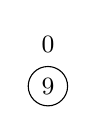
\begin{tikzpicture}\small
\draw (0,0) circle (0.25cm); 
  \node at (0,0) {9};
  \node[anchor=north] at (0,0.75) {0};
\end{tikzpicture}

Step2:

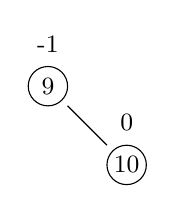
\begin{tikzpicture}\small
\draw (0,0) circle (0.25cm); 
  \node at (0,0) {9};
  \node[anchor=north] at (0,0.75) {-1};
  \draw (1,-1) circle (0.25cm); 
  \node at (1,-1) {10};
  \node[anchor=north] at (1,-0.25) {0};
  \draw (0.25,-0.25)--(0.75,-0.75);
\end{tikzpicture}

Step3:

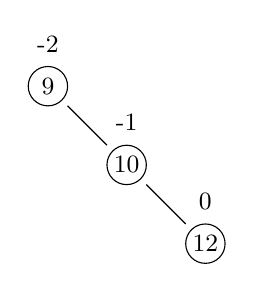
\begin{tikzpicture}\small
\draw (0,0) circle (0.25cm); 
  \node at (0,0) {9};
  \node[anchor=north] at (0,0.75) {-2};
  \draw (1,-1) circle (0.25cm); 
  \node at (1,-1) {10};
  \node[anchor=north] at (1,-0.25) {-1};
  \draw (0.25,-0.25)--(0.75,-0.75);
  \node at (2,-2) {12};
  \draw (2,-2) circle (0.25cm); 
  \draw (1.25,-1.25)--(1.75,-1.75);
  \node[anchor=north] at (2,-1.25) {0};
\end{tikzpicture}

Step4:

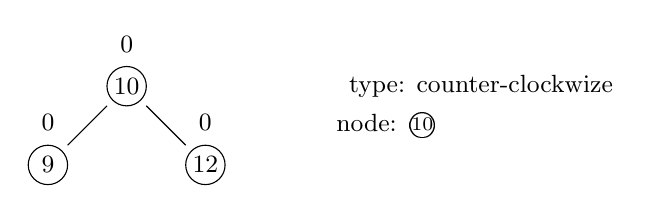
\begin{tikzpicture}\small
\draw (0,0) circle (0.25cm); 
  \node at (0,0) {10};
  \node[anchor=north] at (0,0.75) {0};
  \draw (1,-1) circle (0.25cm); 
  \node at (1,-1) {12};
  \node[anchor=north] at (1,-0.25) {0};
  \draw (0.25,-0.25)--(0.75,-0.75);
  \draw (-1,-1) circle (0.25cm); 
  \node at (-1,-1) {9};
  \node[anchor=north] at (-1,-0.25) {0};
  \draw (-0.25,-0.25)--(-0.75,-0.75);
\node at (4.5,0) {type: counter-clockwize};
\node at (3.3,-0.5) { node: {\small\textcircled{\scriptsize{10}}}};
\end{tikzpicture}

Step5:

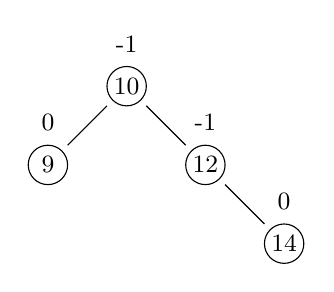
\begin{tikzpicture}\small
\draw (0,0) circle (0.25cm); 
  \node at (0,0) {10};
  \node[anchor=north] at (0,0.75) {-1};
  \draw (1,-1) circle (0.25cm); 
  \node at (1,-1) {12};
  \node[anchor=north] at (1,-0.25) {-1};
  \draw (0.25,-0.25)--(0.75,-0.75);
  \draw (2,-2) circle (0.25cm); 
  \node at (2,-2) {14};
  \node[anchor=north] at (2,-1.25) {0};
  \draw (1.25,-1.25)--(1.75,-1.75);
  \draw (-1,-1) circle (0.25cm); 
  \node at (-1,-1) {9};
  \node[anchor=north] at (-1,-0.25) {0};
  \draw (-0.25,-0.25)--(-0.75,-0.75);
\end{tikzpicture}

Step6:

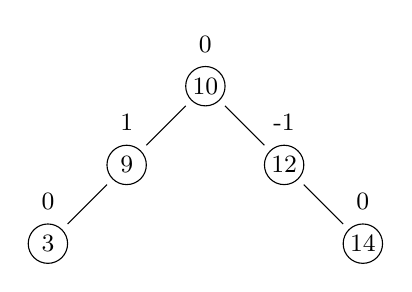
\begin{tikzpicture}\small
\draw (0,0) circle (0.25cm); 
  \node at (0,0) {10};
  \node[anchor=north] at (0,0.75) {0};
  \draw (1,-1) circle (0.25cm); 
  \node at (1,-1) {12};
  \node[anchor=north] at (1,-0.25) {-1};
  \draw (0.25,-0.25)--(0.75,-0.75);
  \draw (2,-2) circle (0.25cm); 
  \node at (2,-2) {14};
  \node[anchor=north] at (2,-1.25) {0};
  \draw (1.25,-1.25)--(1.75,-1.75);
  \draw (-1,-1) circle (0.25cm); 
  \node at (-1,-1) {9};
  \node[anchor=north] at (-1,-0.25) {1};
  \draw (-0.25,-0.25)--(-0.75,-0.75);
   \draw (-2,-2) circle (0.25cm); 
  \node at (-2,-2) {3};
  \node[anchor=north] at (-2,-1.25) {0};
  \draw (-1.25,-1.25)--(-1.75,-1.75);
\end{tikzpicture}

\newpage
Step7:

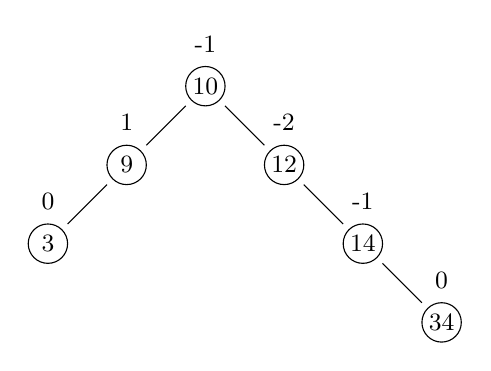
\begin{tikzpicture}\small
\draw (0,0) circle (0.25cm); 
  \node at (0,0) {10};
  \node[anchor=north] at (0,0.75) {-1};
  \draw (1,-1) circle (0.25cm); 
  \node at (1,-1) {12};
  \node[anchor=north] at (1,-0.25) {-2};
  \draw (0.25,-0.25)--(0.75,-0.75);
  \draw (2,-2) circle (0.25cm); 
  \node at (2,-2) {14};
  \node[anchor=north] at (2,-1.25) {-1};
  \draw (1.25,-1.25)--(1.75,-1.75);
  \draw (3,-3) circle (0.25cm); 
  \node at (3,-3) {34};
  \node[anchor=north] at (3,-2.25) {0};
  \draw (2.25,-2.25)--(2.75,-2.75);
  \draw (-1,-1) circle (0.25cm); 
  \node at (-1,-1) {9};
  \node[anchor=north] at (-1,-0.25) {1};
  \draw (-0.25,-0.25)--(-0.75,-0.75);
   \draw (-2,-2) circle (0.25cm); 
  \node at (-2,-2) {3};
  \node[anchor=north] at (-2,-1.25) {0};
  \draw (-1.25,-1.25)--(-1.75,-1.75);
\end{tikzpicture}

Step8:

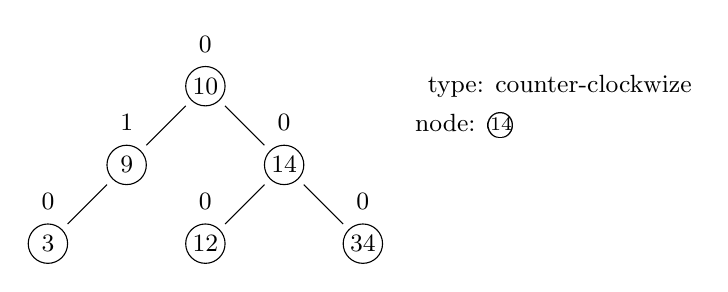
\begin{tikzpicture}\small
\draw (0,0) circle (0.25cm); 
  \node at (0,0) {10};
  \node[anchor=north] at (0,0.75) {0};
  \draw (1,-1) circle (0.25cm); 
  \node at (1,-1) {14};
  \node[anchor=north] at (1,-0.25) {0};
  \draw (0.25,-0.25)--(0.75,-0.75);
  \draw (2,-2) circle (0.25cm); 
  \node at (2,-2) {34};
  \node[anchor=north] at (2,-1.25) {0};
  \draw (1.25,-1.25)--(1.75,-1.75);
  \draw (0,-2) circle (0.25cm); 
  \node at (0,-2) {12};
  \node[anchor=north] at (0,-1.25) {0};
  \draw (0.75,-1.25)--(0.25,-1.75);
  \draw (-1,-1) circle (0.25cm); 
  \node at (-1,-1) {9};
  \node[anchor=north] at (-1,-0.25) {1};
  \draw (-0.25,-0.25)--(-0.75,-0.75);
   \draw (-2,-2) circle (0.25cm); 
  \node at (-2,-2) {3};
  \node[anchor=north] at (-2,-1.25) {0};
  \draw (-1.25,-1.25)--(-1.75,-1.75);
  \node at (4.5,0) {type: counter-clockwize};
\node at (3.3,-0.5) {node: {\small\textcircled{\scriptsize{14}}}};
\end{tikzpicture}

Step9:

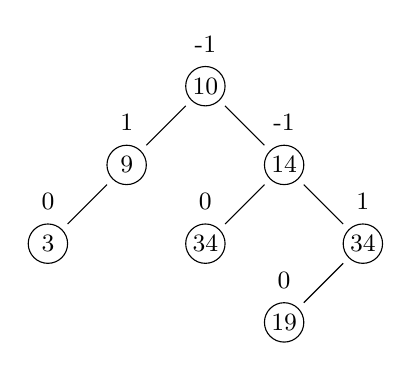
\begin{tikzpicture}\small
\draw (0,0) circle (0.25cm); 
  \node at (0,0) {10};
  \node[anchor=north] at (0,0.75) {-1};
  \draw (1,-1) circle (0.25cm); 
  \node at (1,-1) {14};
  \node[anchor=north] at (1,-0.25) {-1};
  \draw (0.25,-0.25)--(0.75,-0.75);
  \draw (2,-2) circle (0.25cm); 
  \node at (2,-2) {34};
  \node[anchor=north] at (2,-1.25) {1};
  \draw (1.25,-1.25)--(1.75,-1.75);
  \draw (0,-2) circle (0.25cm); 
  \node at (0,-2) {34};
  \node[anchor=north] at (0,-1.25) {0};
  \draw (0.75,-1.25)--(0.25,-1.75);
  \draw (1,-3) circle (0.25cm); 
  \node at (1,-3) {19};
  \node[anchor=north] at (1,-2.25) {0};
  \draw (1.75,-2.25)--(1.25,-2.75);
  \draw (-1,-1) circle (0.25cm); 
  \node at (-1,-1) {9};
  \node[anchor=north] at (-1,-0.25) {1};
  \draw (-0.25,-0.25)--(-0.75,-0.75);
   \draw (-2,-2) circle (0.25cm); 
  \node at (-2,-2) {3};
  \node[anchor=north] at (-2,-1.25) {0};
  \draw (-1.25,-1.25)--(-1.75,-1.75);
\end{tikzpicture}

\newpage
Step10:

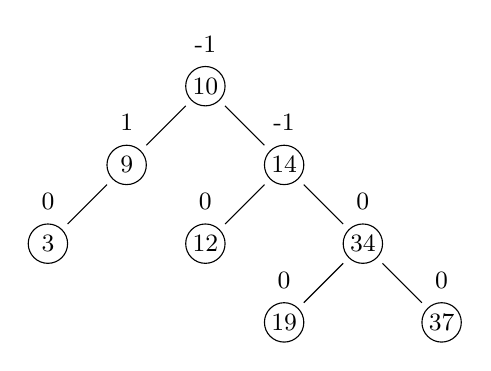
\begin{tikzpicture}\small
\draw (0,0) circle (0.25cm); 
  \node at (0,0) {10};
  \node[anchor=north] at (0,0.75) {-1};
  \draw (1,-1) circle (0.25cm); 
  \node at (1,-1) {14};
  \node[anchor=north] at (1,-0.25) {-1};
  \draw (0.25,-0.25)--(0.75,-0.75);
  \draw (2,-2) circle (0.25cm); 
  \node at (2,-2) {34};
  \node[anchor=north] at (2,-1.25) {0};
  \draw (1.25,-1.25)--(1.75,-1.75);
  \draw (3,-3) circle (0.25cm); 
  \node at (3,-3) {37};
  \node[anchor=north] at (3,-2.25) {0};
  \draw (2.25,-2.25)--(2.75,-2.75);
  \draw (0,-2) circle (0.25cm); 
  \node at (0,-2) {12};
  \node[anchor=north] at (0,-1.25) {0};
  \draw (0.75,-1.25)--(0.25,-1.75);
  \draw (1,-3) circle (0.25cm); 
  \node at (1,-3) {19};
  \node[anchor=north] at (1,-2.25) {0};
  \draw (1.75,-2.25)--(1.25,-2.75);
  \draw (-1,-1) circle (0.25cm); 
  \node at (-1,-1) {9};
  \node[anchor=north] at (-1,-0.25) {1};
  \draw (-0.25,-0.25)--(-0.75,-0.75);
   \draw (-2,-2) circle (0.25cm); 
  \node at (-2,-2) {3};
  \node[anchor=north] at (-2,-1.25) {0};
  \draw (-1.25,-1.25)--(-1.75,-1.75);
\end{tikzpicture}


Step11:

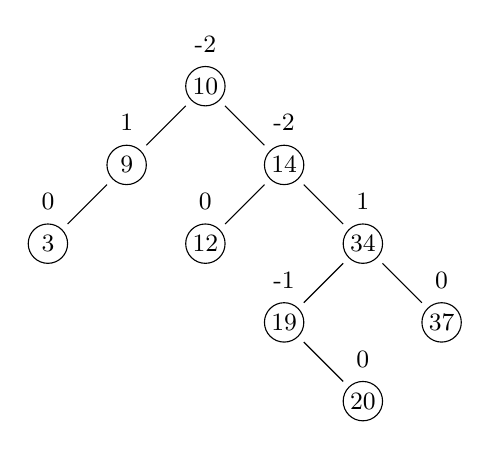
\begin{tikzpicture}\small
\draw (0,0) circle (0.25cm); 
  \node at (0,0) {10};
  \node[anchor=north] at (0,0.75) {-2};
  \draw (1,-1) circle (0.25cm); 
  \node at (1,-1) {14};
  \node[anchor=north] at (1,-0.25) {-2};
  \draw (0.25,-0.25)--(0.75,-0.75);
  \draw (2,-2) circle (0.25cm); 
  \node at (2,-2) {34};
  \node[anchor=north] at (2,-1.25) {1};
  \draw (1.25,-1.25)--(1.75,-1.75);
  \draw (3,-3) circle (0.25cm); 
  \node at (3,-3) {37};
  \node[anchor=north] at (3,-2.25) {0};
  \draw (2.25,-2.25)--(2.75,-2.75);
  \draw (0,-2) circle (0.25cm); 
  \node at (0,-2) {12};
  \node[anchor=north] at (0,-1.25) {0};
  \draw (0.75,-1.25)--(0.25,-1.75);
  \draw (1,-3) circle (0.25cm); 
  \node at (1,-3) {19};
  \node[anchor=north] at (1,-2.25) {-1};
  \draw (1.75,-2.25)--(1.25,-2.75);
  \draw (2,-4) circle (0.25cm); 
  \node at (2,-4) {20};
  \node[anchor=north] at (2,-3.25) {0};
  \draw (1.25,-3.25)--(1.75,-3.75);
  \draw (-1,-1) circle (0.25cm); 
  \node at (-1,-1) {9};
  \node[anchor=north] at (-1,-0.25) {1};
  \draw (-0.25,-0.25)--(-0.75,-0.75);
   \draw (-2,-2) circle (0.25cm); 
  \node at (-2,-2) {3};
  \node[anchor=north] at (-2,-1.25) {0};
  \draw (-1.25,-1.25)--(-1.75,-1.75);
\end{tikzpicture}


Step12:

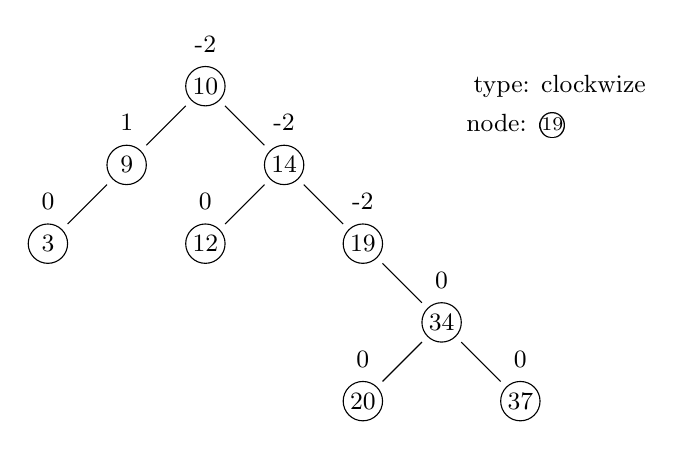
\begin{tikzpicture}\small
\draw (0,0) circle (0.25cm); 
  \node at (0,0) {10};
  \node[anchor=north] at (0,0.75) {-2};
  \draw (1,-1) circle (0.25cm); 
  \node at (1,-1) {14};
  \node[anchor=north] at (1,-0.25) {-2};
  \draw (0.25,-0.25)--(0.75,-0.75);
  \draw (2,-2) circle (0.25cm); 
  \node at (2,-2) {19};
  \node[anchor=north] at (2,-1.25) {-2};
  \draw (1.25,-1.25)--(1.75,-1.75);
  \draw (3,-3) circle (0.25cm); 
  \node at (3,-3) {34};
  \node[anchor=north] at (3,-2.25) {0};
  \draw (2.25,-2.25)--(2.75,-2.75);
  \draw (0,-2) circle (0.25cm); 
  \node at (0,-2) {12};
  \node[anchor=north] at (0,-1.25) {0};
  \draw (0.75,-1.25)--(0.25,-1.75);
  \draw (2,-4) circle (0.25cm); 
  \node at (2,-4) {20};
  \node[anchor=north] at (2,-3.25) {0};
  \draw (2.75,-3.25)--(2.25,-3.75);
  \draw (-1,-1) circle (0.25cm); 
  \node at (-1,-1) {9};
  \node[anchor=north] at (-1,-0.25) {1};
  \draw (-0.25,-0.25)--(-0.75,-0.75);
   \draw (-2,-2) circle (0.25cm); 
  \node at (-2,-2) {3};
  \node[anchor=north] at (-2,-1.25) {0};
  \draw (-1.25,-1.25)--(-1.75,-1.75);
  \draw (4,-4) circle (0.25cm); 
  \node at (4,-4) {37};
  \node[anchor=north] at (4,-3.25) {0};
  \draw (3.25,-3.25)--(3.75,-3.75);
  \node at (4.5,0) {type: clockwize};
\node at (3.95,-0.5) {node: {\small\textcircled{\scriptsize{19}}}};
\end{tikzpicture}

\newpage
Step13:

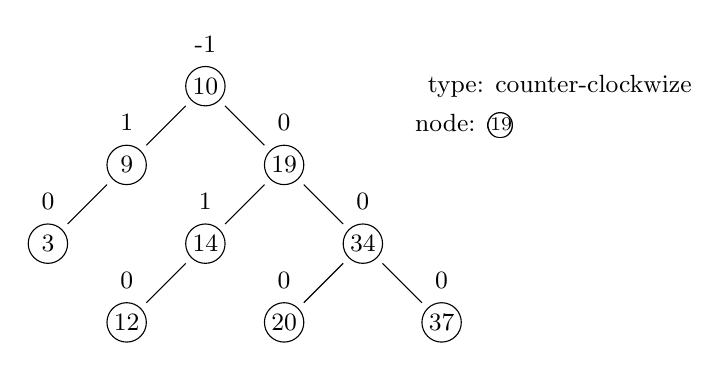
\begin{tikzpicture}\small
\draw (0,0) circle (0.25cm); 
  \node at (0,0) {10};
  \node[anchor=north] at (0,0.75) {-1};
  \draw (1,-1) circle (0.25cm); 
  \node at (1,-1) {19};
  \node[anchor=north] at (1,-0.25) {0};
  \draw (0.25,-0.25)--(0.75,-0.75);
  \draw (2,-2) circle (0.25cm); 
  \node at (2,-2) {34};
  \node[anchor=north] at (2,-1.25) {0};
  \draw (1.25,-1.25)--(1.75,-1.75);
  \draw (3,-3) circle (0.25cm); 
  \node at (3,-3) {37};
  \node[anchor=north] at (3,-2.25) {0};
  \draw (2.25,-2.25)--(2.75,-2.75);
  \draw (0,-2) circle (0.25cm); 
  \node at (0,-2) {14};
  \node[anchor=north] at (0,-1.25) {1};
  \draw (0.75,-1.25)--(0.25,-1.75);
  \draw (-1,-3) circle (0.25cm); 
  \node at (-1,-3) {12};
  \node[anchor=north] at (-1,-2.25) {0};
  \draw (-0.25,-2.25)--(-0.75,-2.75);
  \draw (1,-3) circle (0.25cm); 
  \node at (1,-3) {20};
  \node[anchor=north] at (1,-2.25) {0};
  \draw (1.75,-2.25)--(1.25,-2.75);
  \draw (-1,-1) circle (0.25cm); 
  \node at (-1,-1) {9};
  \node[anchor=north] at (-1,-0.25) {1};
  \draw (-0.25,-0.25)--(-0.75,-0.75);
   \draw (-2,-2) circle (0.25cm); 
  \node at (-2,-2) {3};
  \node[anchor=north] at (-2,-1.25) {0};
  \draw (-1.25,-1.25)--(-1.75,-1.75);
  \node at (4.5,0)  {type: counter-clockwize};
\node at (3.3,-0.5) {node: {\small\textcircled{\scriptsize{19}}}};
\end{tikzpicture}

2. Step1:

\begin{tikzpicture}\small
\draw (-1,1) circle (0.25cm); 
  \node at (-1,1) {8};
  \node[anchor=north] at (-1,1.75) {1};
  \draw (-0.75,0.75)--(0.75,-0.75);
  \draw (1,-1) circle (0.25cm); 
  \node at (1,-1) {11};
  \node[anchor=north] at (1,-0.25) {0};
  \draw (1.25,-1.25)--(1.75,-1.75);
  \draw (2,-2) circle (0.25cm); 
  \node at (2,-2) {13};
  \node[anchor=north] at (2,-1.25) {0};
  \draw (2.25,-2.25)--(2.75,-2.75);
  \draw (3,-3) circle (0.25cm); 
  \node at (3,-3) {14};
  \node[anchor=north] at (3,-2.25) {0};
  \draw (0.75,-1.25)--(0.25,-1.75);
  \draw (0,-2) circle (0.25cm); 
  \node at (0,-2) {10};
  \node[anchor=north] at (0,-1.25) {1};
   \draw (-0.25,-2.25)--(-0.75,-2.75);
  \draw (-1,-3) circle (0.25cm); 
  \node at (-1,-3) {9};
  \node[anchor=north] at (-1,-2.25) {0};
  \draw (1.75,-2.25)--(1.25,-2.75);
  \draw (1,-3) circle (0.25cm); 
  \node at (1,-3) {12};
  \node[anchor=north] at (1,-2.25) {0};
  \draw (-1.25,0.75)--(-2.75,-0.75);
  \draw (-3,-1) circle (0.25cm); 
  \node at (-3,-1) {5};
  \node[anchor=north] at (-3,-0.25) {1};
  \draw (-2.75,-1.25)--(-2.25,-1.75);
  \draw (-2,-2) circle (0.25cm); 
  \node at (-2,-2) {7};
  \node[anchor=north] at (-2,-1.25) {1};
\draw (-2.25,-2.25)--(-2.75,-2.75);
  \draw (-3,-3) circle (0.25cm); 
  \node at (-3,-3) {6};
  \node[anchor=north] at (-3,-2.25) {0};
\draw (-3.25,-1.25)--(-4.75,-2.75);
  \draw (-5,-3) circle (0.25cm); 
  \node at (-5,-3) {3};
  \node[anchor=north] at (-5,-2.25) {1};
\draw (-4.75,-3.25)--(-4.25,-3.75);
  \draw (-4,-4) circle (0.25cm); 
  \node at (-4,-4) {4};
  \node[anchor=north] at (-4,-3.25) {0};
\draw (-5.25,-3.25)--(-5.75,-3.75);
  \draw (-6,-4) circle (0.25cm); 
  \node at (-6,-4) {1};
  \node[anchor=north] at (-6,-3.25) {1};
\draw (-6.25,-4.25)--(-6.75,-4.75);
  \draw (-7,-5) circle (0.25cm); 
  \node at (-7,-5) {0};
  \node[anchor=north] at (-7,-4.25) {0}; 
\end{tikzpicture}

Step2:

\begin{tikzpicture}\small
\draw (-1,1) circle (0.25cm); 
  \node at (-1,1) {8};
  \node[anchor=north] at (-1,1.75) {1};
  \draw (-0.75,0.75)--(0.75,-0.75);
  \draw (1,-1) circle (0.25cm); 
  \node at (1,-1) {12};
  \node[anchor=north] at (1,-0.25) {0};
  \draw (1.25,-1.25)--(1.75,-1.75);
  \draw (2,-2) circle (0.25cm); 
  \node at (2,-2) {13};
  \node[anchor=north] at (2,-1.25) {-1};
  \draw (2.25,-2.25)--(2.75,-2.75);
  \draw (3,-3) circle (0.25cm); 
  \node at (3,-3) {14};
  \node[anchor=north] at (3,-2.25) {0};
  \draw (0.75,-1.25)--(0.25,-1.75);
  \draw (0,-2) circle (0.25cm); 
  \node at (0,-2) {10};
  \node[anchor=north] at (0,-1.25) {1};
   \draw (-0.25,-2.25)--(-0.75,-2.75);
  \draw (-1,-3) circle (0.25cm); 
  \node at (-1,-3) {9};
  \node[anchor=north] at (-1,-2.25) {0};
  \draw (-1.25,0.75)--(-2.75,-0.75);
  \draw (-3,-1) circle (0.25cm); 
  \node at (-3,-1) {5};
  \node[anchor=north] at (-3,-0.25) {1};
  \draw (-2.75,-1.25)--(-2.25,-1.75);
  \draw (-2,-2) circle (0.25cm); 
  \node at (-2,-2) {7};
  \node[anchor=north] at (-2,-1.25) {1};
\draw (-2.25,-2.25)--(-2.75,-2.75);
  \draw (-3,-3) circle (0.25cm); 
  \node at (-3,-3) {6};
  \node[anchor=north] at (-3,-2.25) {0};
\draw (-3.25,-1.25)--(-4.75,-2.75);
  \draw (-5,-3) circle (0.25cm); 
  \node at (-5,-3) {3};
  \node[anchor=north] at (-5,-2.25) {1};
\draw (-4.75,-3.25)--(-4.25,-3.75);
  \draw (-4,-4) circle (0.25cm); 
  \node at (-4,-4) {4};
  \node[anchor=north] at (-4,-3.25) {0};
\draw (-5.25,-3.25)--(-5.75,-3.75);
  \draw (-6,-4) circle (0.25cm); 
  \node at (-6,-4) {1};
  \node[anchor=north] at (-6,-3.25) {1};
\draw (-6.25,-4.25)--(-6.75,-4.75);
  \draw (-7,-5) circle (0.25cm); 
  \node at (-7,-5) {0};
  \node[anchor=north] at (-7,-4.25) {0}; 
\end{tikzpicture}

Step3:

\begin{tikzpicture}\small
\draw (-1,1) circle (0.25cm); 
  \node at (-1,1) {8};
  \node[anchor=north] at (-1,1.75) {1};
  \draw (-0.75,0.75)--(0.75,-0.75);
  \draw (1,-1) circle (0.25cm); 
  \node at (1,-1) {13};
  \node[anchor=north] at (1,-0.25) {1};
  \draw (1.25,-1.25)--(1.75,-1.75);
  \draw (2,-2) circle (0.25cm); 
  \node at (2,-2) {14};
  \node[anchor=north] at (2,-1.25) {0};
  \draw (0.75,-1.25)--(0.25,-1.75);
  \draw (0,-2) circle (0.25cm); 
  \node at (0,-2) {10};
  \node[anchor=north] at (0,-1.25) {1};
   \draw (-0.25,-2.25)--(-0.75,-2.75);
  \draw (-1,-3) circle (0.25cm); 
  \node at (-1,-3) {9};
  \node[anchor=north] at (-1,-2.25) {0};
  \draw (-1.25,0.75)--(-2.75,-0.75);
  \draw (-3,-1) circle (0.25cm); 
  \node at (-3,-1) {5};
  \node[anchor=north] at (-3,-0.25) {1};
  \draw (-2.75,-1.25)--(-2.25,-1.75);
  \draw (-2,-2) circle (0.25cm); 
  \node at (-2,-2) {7};
  \node[anchor=north] at (-2,-1.25) {1};
\draw (-2.25,-2.25)--(-2.75,-2.75);
  \draw (-3,-3) circle (0.25cm); 
  \node at (-3,-3) {6};
  \node[anchor=north] at (-3,-2.25) {0};
\draw (-3.25,-1.25)--(-4.75,-2.75);
  \draw (-5,-3) circle (0.25cm); 
  \node at (-5,-3) {3};
  \node[anchor=north] at (-5,-2.25) {1};
\draw (-4.75,-3.25)--(-4.25,-3.75);
  \draw (-4,-4) circle (0.25cm); 
  \node at (-4,-4) {4};
  \node[anchor=north] at (-4,-3.25) {0};
\draw (-5.25,-3.25)--(-5.75,-3.75);
  \draw (-6,-4) circle (0.25cm); 
  \node at (-6,-4) {1};
  \node[anchor=north] at (-6,-3.25) {1};
\draw (-6.25,-4.25)--(-6.75,-4.75);
  \draw (-7,-5) circle (0.25cm); 
  \node at (-7,-5) {0};
  \node[anchor=north] at (-7,-4.25) {0}; 
\end{tikzpicture}

Step4:

\begin{tikzpicture}\small
\draw (-1,1) circle (0.25cm); 
  \node at (-1,1) {8};
  \node[anchor=north] at (-1,1.75) {1};
  \draw (-0.75,0.75)--(0.75,-0.75);
  \draw (1,-1) circle (0.25cm); 
  \node at (1,-1) {14};
  \node[anchor=north] at (1,-0.25) {2};
  \draw (0.75,-1.25)--(0.25,-1.75);
  \draw (0,-2) circle (0.25cm); 
  \node at (0,-2) {10};
  \node[anchor=north] at (0,-1.25) {1};
   \draw (-0.25,-2.25)--(-0.75,-2.75);
  \draw (-1,-3) circle (0.25cm); 
  \node at (-1,-3) {9};
  \node[anchor=north] at (-1,-2.25) {0};
  \draw (-1.25,0.75)--(-2.75,-0.75);
  \draw (-3,-1) circle (0.25cm); 
  \node at (-3,-1) {5};
  \node[anchor=north] at (-3,-0.25) {1};
  \draw (-2.75,-1.25)--(-2.25,-1.75);
  \draw (-2,-2) circle (0.25cm); 
  \node at (-2,-2) {7};
  \node[anchor=north] at (-2,-1.25) {1};
\draw (-2.25,-2.25)--(-2.75,-2.75);
  \draw (-3,-3) circle (0.25cm); 
  \node at (-3,-3) {6};
  \node[anchor=north] at (-3,-2.25) {0};
\draw (-3.25,-1.25)--(-4.75,-2.75);
  \draw (-5,-3) circle (0.25cm); 
  \node at (-5,-3) {3};
  \node[anchor=north] at (-5,-2.25) {1};
\draw (-4.75,-3.25)--(-4.25,-3.75);
  \draw (-4,-4) circle (0.25cm); 
  \node at (-4,-4) {4};
  \node[anchor=north] at (-4,-3.25) {0};
\draw (-5.25,-3.25)--(-5.75,-3.75);
  \draw (-6,-4) circle (0.25cm); 
  \node at (-6,-4) {1};
  \node[anchor=north] at (-6,-3.25) {1};
\draw (-6.25,-4.25)--(-6.75,-4.75);
  \draw (-7,-5) circle (0.25cm); 
  \node at (-7,-5) {0};
  \node[anchor=north] at (-7,-4.25) {0}; 
\end{tikzpicture}

\newpage
Step5:

\begin{tikzpicture}\small
\draw (-1,1) circle (0.25cm); 
  \node at (-1,1) {8};
  \node[anchor=north] at (-1,1.75) {2};
  \draw (-0.75,0.75)--(0.75,-0.75);
  \draw (1,-1) circle (0.25cm); 
  \node at (1,-1) {10};
  \node[anchor=north] at (1,-0.25) {0};
  \draw (1.25,-1.25)--(1.75,-1.75);
  \draw (2,-2) circle (0.25cm); 
  \node at (2,-2) {14};
  \node[anchor=north] at (2,-1.25) {0};
  \draw (0.75,-1.25)--(0.25,-1.75);
  \draw (0,-2) circle (0.25cm); 
  \node at (0,-2) {9};
  \node[anchor=north] at (0,-1.25) {0};
  \draw (-1.25,0.75)--(-2.75,-0.75);
  \draw (-3,-1) circle (0.25cm); 
  \node at (-3,-1) {5};
  \node[anchor=north] at (-3,-0.25) {1};
  \draw (-2.75,-1.25)--(-2.25,-1.75);
  \draw (-2,-2) circle (0.25cm); 
  \node at (-2,-2) {7};
  \node[anchor=north] at (-2,-1.25) {1};
\draw (-2.25,-2.25)--(-2.75,-2.75);
  \draw (-3,-3) circle (0.25cm); 
  \node at (-3,-3) {6};
  \node[anchor=north] at (-3,-2.25) {0};
\draw (-3.25,-1.25)--(-4.75,-2.75);
  \draw (-5,-3) circle (0.25cm); 
  \node at (-5,-3) {3};
  \node[anchor=north] at (-5,-2.25) {1};
\draw (-4.75,-3.25)--(-4.25,-3.75);
  \draw (-4,-4) circle (0.25cm); 
  \node at (-4,-4) {4};
  \node[anchor=north] at (-4,-3.25) {0};
\draw (-5.25,-3.25)--(-5.75,-3.75);
  \draw (-6,-4) circle (0.25cm); 
  \node at (-6,-4) {1};
  \node[anchor=north] at (-6,-3.25) {1};
\draw (-6.25,-4.25)--(-6.75,-4.75);
  \draw (-7,-5) circle (0.25cm); 
  \node at (-7,-5) {0};
  \node[anchor=north] at (-7,-4.25) {0}; 
  \node at (4.5,0) {type: clockwize};
\node at (3.95,-0.5) {node: {\small\textcircled{\scriptsize{10}}}};
\end{tikzpicture}


Step6:

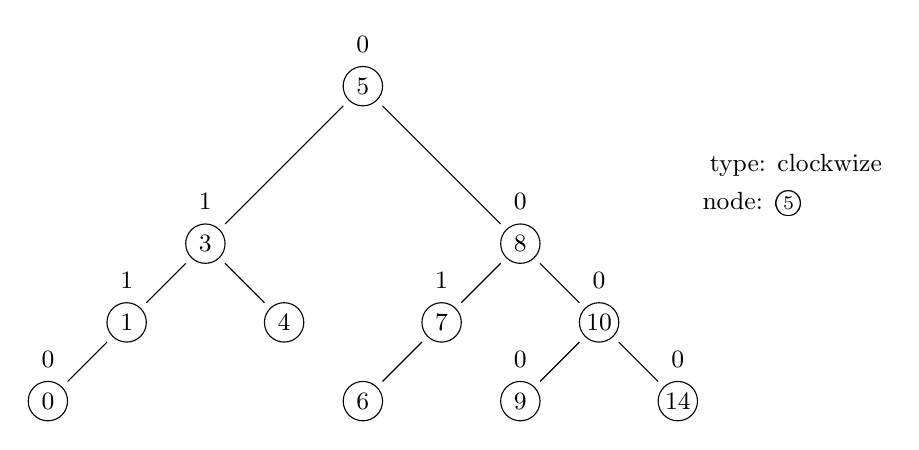
\begin{tikzpicture}\small
\draw (-1,1) circle (0.25cm); 
  \node at (-1,1) {5};
  \node[anchor=north] at (-1,1.75) {0};
  \draw (-0.75,0.75)--(0.75,-0.75);
  \draw (1,-1) circle (0.25cm); 
  \node at (1,-1) {8};
  \node[anchor=north] at (1,-0.25) {0};
  \draw (1.25,-1.25)--(1.75,-1.75);
  \draw (2,-2) circle (0.25cm); 
  \node at (2,-2) {10};
  \node[anchor=north] at (2,-1.25) {0};
  \draw (2.25,-2.25)--(2.75,-2.75);
  \draw (3,-3) circle (0.25cm); 
  \node at (3,-3) {14};
  \node[anchor=north] at (3,-2.25) {0};
  \draw (0.75,-1.25)--(0.25,-1.75);
  \draw (0,-2) circle (0.25cm); 
  \node at (0,-2) {7};
  \node[anchor=north] at (0,-1.25) {1};
   \draw (-0.25,-2.25)--(-0.75,-2.75);
  \draw (-1,-3) circle (0.25cm); 
  \node at (-1,-3) {6};
  \node[anchor=north] at (-1,-2.25) {};
  \draw (1.75,-2.25)--(1.25,-2.75);
  \draw (1,-3) circle (0.25cm); 
  \node at (1,-3) {9};
  \node[anchor=north] at (1,-2.25) {0};
  \draw (-1.25,0.75)--(-2.75,-0.75);
  \draw (-3,-1) circle (0.25cm); 
  \node at (-3,-1) {3};
  \node[anchor=north] at (-3,-0.25) {1};
\draw (-2.75,-1.25)--(-2.25,-1.75);
  \draw (-2,-2) circle (0.25cm); 
  \node at (-2,-2) {4};
  \node[anchor=north] at (-2,-1.25) {};
\draw (-3.25,-1.25)--(-3.75,-1.75);
  \draw (-4,-2) circle (0.25cm); 
  \node at (-4,-2) {1};
  \node[anchor=north] at (-4,-1.25) {1}; 
\draw (-4.25,-2.25)--(-4.75,-2.75);
  \draw (-5,-3) circle (0.25cm); 
  \node at (-5,-3) {0};
  \node[anchor=north] at (-5,-2.25) {0};
  \node at (4.5,0) {type: clockwize};
  \node at (3.95,-0.5) {node: {\small\textcircled{\scriptsize{5}}}};
\end{tikzpicture}
\newpage

Q4

1.

The node  S has: 

\#key: the left end point x of interval [x, y]

\#right\_end: the right end point y of interval [x, y] 

\#height: the height of the tree whose root is S

\#max\_y: the max value of y in the tree whose root is S

\#left: the left node

\#right: the right node

2.

For the rebalance mentioned below, we need to add update\_height and update\_max\_y functions in the end of each single and double rotation by using the course rebalance algorithm.
\begin{verbatim}
update_height(S) -- pseudocode
if S == nil:
    return
if S.left == nil and S.right == nil:
    S.height = 1
    return
if S.left == nil and S.right != nil:
    S.height = S.right.height + 1
    return
if S.left != nil and S.right == nil:
    S.height = S.left.height + 1
    return
S.height = max(S.left.height, S.right.height) + 1
return
\end{verbatim}

\begin{verbatim}
update_max_y(S) -- pseudocode
if S == nil:
    return
if S.left == nil and S.right == nil:
    S.max_y = S.right_end
    return
if S.left == nil and S.right != nil:
    S.max_y = max(S.right.max_y, S.right_end)
    return
if S.left != nil and S.right == nil:
    S.max_y = max(S.left.max_y, S.right_end)
    return
S.max_y = max(S.left.max_y, S.right.max_y, S.right_end)
return
\end{verbatim}

\begin{verbatim}
insert(S, x, y) -- pseudocode
if S == nil:
    S = new node(key=x, right_end=y, height=1, max_y=y, left=nil, right=nil)
    return S
if S.key == x and S.right_end == y:
    return S
if S.key > x:
    S.left = insert(S.left, x, y)
    update_height(S)
    update_max_y(S)
    rebalance at S
    return S
else:
    S.right = insert(S.right, x, y)
    update_height(S)
    update_max_y(S)
    rebalance at S
    return S   
\end{verbatim}

\begin{verbatim}
delete(S, x, y) -- pseudocode
if S == nil:
    return nil
if S.key == x and S.right_end == y:
    if S.left == nil:
        return S.right
    if S.right == nil:
        return S.left;
    search from S.right to the left most node p of the right subtree of S
    S.key = q.key
    S.right_end = q.right_end
    S.right = delete(S.right, q.key, q.right_end)
    update_height(S)
    update_max_y(S)
    rebalance at S
    return S
if S.key > x:
    S.left = delete(S.left, x, y)
    update_height(S)
    update_max_y(S)
    rebalance at S
    return S
S.right = delete(S.right, x, y)
update_height(S)
update_max_y(S)
rebalance at S
return S
\end{verbatim}

\begin{verbatim}
eclipse(S, l, h) -- pseudocode
if S == nil or S.max_y <= l:
    return None
if l <= S.key and S.right_end <= h:
    return [S.key, S.right_end]
if S.left != nil and S.left.max_y > l:
    interval = eclipse(S.left, l, h)
    if interval == None:
        if S.right == nil or S.right.max_y <= l:
            return None
        return eclipse(S.right, l, h)
    return interval
return eclipse(S.right, l, h)
\end{verbatim}

3.

For insert and delete, my algorithm is based on insert and delete operations of BST(i.e. I only search in one sub-tree), whose complexity is $O{\left(log(n)\right)}$ if the tree with root S is AVL with height $log(n)$.
Also my update functions for height and max\_y are with complexity $O{\left(1\right)}$, so the whole complexity is $O{\left(log(n)\right)}$. Also,as I have helper function for updating height and max\_y, similar insert and delete approaches to BST and the use of rebalanced, my algorithms is right. By the way, I first update height and then rebalanced the tree, which let all nodes have correct balance factors. At last, I update the max\_y based on new AVL.

For eclipse, in base case I consider the easiest cases that must have and must not have, with complexity $O{\left(1\right)}$, then I consider cases that the sub-trees of S may have such interval. I first search on left sub-tree and return if find(similar to search in BST), the complexity is $O{\left(log(n)\right)}$. If I can not find, then I goes to the right sub-tree with similar approach, also 
with $O{\left(log(n)\right)}$ complexity. So in worst case, my complexity is $O{\left(log(n)\right)} + O{\left(log(n)\right)}$ which is still $O{\left(log(n)\right)}$. As I have consider from base cases to all sub-tree cases, my algorithm is correct.
\end{document}